% !TEX root = ../Tesis_NataliaOpazo.tex

 A continuación se presenta la estructura de este trabajo para comprender la interacción entre la productividad biológica, la biogeoquímica y el clima. Se utilizó para ello un modelo del ciclo del carbono con una representación del ciclo biogeoquímico del océano, durante el periodo correspondiente a la transición del Pleistoceno al Holoceno. Para lo cual se presentan los flujos de campo de polvo, provenientes tanto de reconstrucciones como de modelos simulados. El trabajo estará enfocado en cuantificar los efectos del ciclo biogeoquímico del hierro en la bomba de tejidos blandos, relacionándolo con la captura del CO$_2$ tanto a global como en las zonas HNLC. 

 Para poder responder al objetivo general, este trabajo seguirá la siguiente estructura: 

\begin{itemize}
\item[\bf I.] Tratamiento del modelo cGENIE al ciclo del hierro oceánico (sección 4.1).
\item[\bf II.] Se presenta la fuente de los datos (sección 4.2). Las que nos describen la cantidad de fuentes de polvo en ambos periodos UMG y Holoceno.  
\item[\bf III.] Pre-procesamiento de los datos (sección 4.3). Se editan las fuentes de polvo con el objeto de dejarlas como input para el modelo cGENIE. 
\item[\bf IIII.] Procesamiento (sección 4.4). Se simulan las fuentes de polvo con el propósito de ver el efecto del hierro en la captura de CO$_2$. 
\end{itemize} \newpage

 \section{Modelo cGENIE}
En este estudio se utilizó un código versión ``muffin'' del \textit{cGENIE Earth system Model of Intermediate Complexity}, en su versión 0.9 (genie.seao2.or). Este modelo fue construido a partir del \textit{Grid ENabled Integrated Earth system model} GENIE, siendo una simplificada versión centrada en el ciclo del carbono \citep{ridgwell2007marine}. En este estudio se usa una versión GENIE que contiene una atmósfera simplificada y que se encuentra centrada en el ciclo del carbono, conocida como cGENIE. Utilizada comúnmente para conocer las interacciones entre la productividad biológica, la biogeoquímica y el clima. Como todo EMIC, este modelo contiene distintas componentes del sistema Tierra. Incorpora representación de la circulación oceánica, biogeoquímica marina, sedimentos del fondo marino y geoquímica \citep{lenton2007effects}. No obstante, el modelo tiene una baja resolución espacial, y una discreta resolución temporal realizando simulaciones de una escala entre 10$^4$ y 10$^5$ años \citep{meyer2016influence} relevante para procesos de retroalimentación biogeoquímica, lo que hace que sea extremadamente eficiente \citep{edwards2005uncertainties}. 

El modelo GENIE-1 contiene 49 trazadores disueltos, propiedades isotópicas importantes en un contexto de cambio climático y estudios paleo, y relaciones molares (si las hay) en sedimentos sólidos y gases atmosféricos. El presente modelo es utilizado con el prop\'osito de conocer los escenarios pasados de pCO$_2$ atmosf\'erico, basado en el impacto de la fertilizaci\'on con hierro procedente de los flujos de polvo a\'ereos en la ecolog\'ia marina. Es por esta razón, que se define el uso de los siguientes trazadores atmosféricos: CO$_2$, $^{13}$C, O$_2$, con la adición de la temperatura y humedad de la atmósfera. Mientras que para el océano: carbono inorgánico total disuelto (DIC), alcalinidad (ALK), fosfato (PO$_4$), hierro (Fe), Oxígeno (O$_2$), las componentes de carbono, fósforo y hierro de materia orgánica disuelta, isótopos estables ($^{13}$C) asociadas al DIC y al DOM, ligandos limitados por hierro, ligandos libres (que pueden enlazarse con hierro). 

Se calcula la redistribución de la concentración de trazadores que no son transportados debido a la circulación oceánica. Así, se ve que la remoción de la solución de nutrientes (PO$_4$ y Fe), el DIC y al alkalinidad, entre otros, ocurre mediante la captación por la productividad biológica en la zona eufótica del océano. Habrá entonces una exportación resultante de material particulado que dependerá de los procesos de remineralización, que eventualmente podrían constituir una nueva solución inorgánica, pero esta vez, a mayor profundidad en comparación de donde los trazadores fueron retirados originalmente. 

Los módulos utilizados para llevar este proceso a cabo son: 

\begin{table}[H]
\centering
\begin{tabular}{|l|l|l|}
\hline
Componente& Abreviatura & Modelo \\
\hline \hline
Atmósfera & eb& EMBM (2-D) \\ \hline
Océano & go & GOLDSTEIN \\ \hline
Cubierta de hielo oceánica &gs& GOLDSTEIN (opciones multiples)  \\ \hline
Química atmosférica&ac&ATCHEM\\\hline
Biogeoquímica oceánica&bg&BIOGEM\\ \hline
\end{tabular}
\caption[Componentes modelo cGENIE]{Detalle de los modelos utilizados y las cacacter\'isticas asociadas a los campos de hierro globales}
\label{tabla:Met1}
\end{table}

\begin{description}

\item{\bf C-GOLDSTEIN}

Módulo que contiene la componente climática y de la física oceánica. Entre sus características incluye una fricción geostrófica reducida, un modelo 3-D de circulación oceánica acoplada, un modelo 2-D de balance de energía-humedad de la atmósfera (EMBM) y un modelo de dinámica-termodinámica del hielo marino \citep{edwards2005uncertainties}.

\item{\bf BIOGEM (BIOGEochemical Model)}

Modulo que se encuentra compuesto y maneja el intercambio gaseoso océano-atmósfera, y la transformación y redistribución espacial de los componentes biogeoquímicos tanto en la superficie (captura biológica) como en el interior del océano (remineralización) \citep{ridgwell2007regulation}. 

\end{description}

 \section{Base de datos}

Entre la base de datos utilizadas se encuentra una reconstrucción y cuatro modelos de polvo (ver secci\'on 2.2) para el periodo del Último Máximo Glacial y el periodo preindustrial. 

A continuaci\'on se presentan la reconstrucci\'on y modelos utilizados.

\subsection{Reconstrucción}

 {\bf Lambert.} Los flujos de depositación de polvo presentados a continuación, corresponden a una reconstrucción basada en datos obtenidos del \textit{Dust Indicators and Records of Terrestrial and Marine Paleoenvironments} (DIRTMAP) en su tercera fase. DIRTMAP es un registro de datos geológicos compilados en la forma de un set de datos espacializados \citep{kohfeld2001dirtmap}, creados con el fin de servir como evaluación para simulaciones desarrolladas con modelos del sistema Tierra que incluyan una componente del ciclo de polvo. 

Esta base de datos fue previamente seleccionada por \cite{lambert2015dust}, que extrajo dos periodos que corresponden al preindustrial y UMG con el propósito de realizar una interpolación espacial, usando para ello el algoritmo de Kriging (para subsanar los lugares sin datos).

\begin{figure}[H]
\centering
 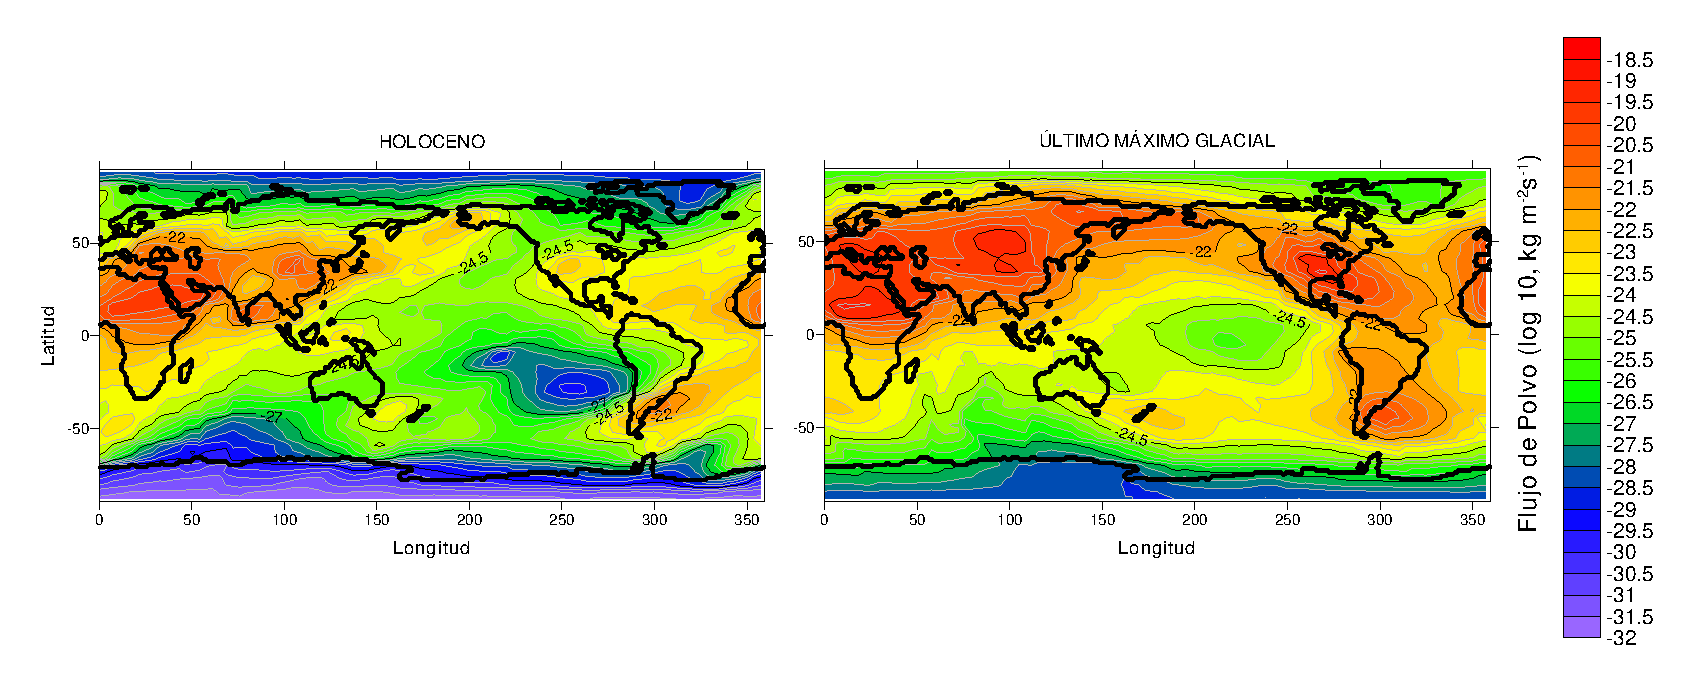
\includegraphics[width=1.1\textwidth]{Plot1_Lambert_2.pdf}
 \caption[Flujos de polvo \cite{lambert2015dust}]{Mapa global de flujos de polvo interpolados entre el periodo del Holoceno y el \'Ultimo M\'aximo Glacial. Datos obtenidos de \cite{lambert2015dust}.}
  \label{fig:Mapa_Lambert}\end{figure}

Los datos muestran que los flujos de depositaciones globales son distintos en los periodos presentados, dado que tanto para el Holoceno como UMG corresponden a 2278.559 Tg año$^{-1}$ y 7639.490 Tg año$^{-1}$ respectivamente. Entre las diferencias que se pueden apreciar entre ambos periodos, es que las fuentes de polvo se intensifican en el UMG en comparación al Holoceno. Así, durante el UMG las fuentes de América (norte y sur) son más pronunciadas y la mayor parte de la deposición en el océano Atlántico Norte parece provenir de América del Norte y de África del Norte por sobre Asia como se muestra durante el Holoceno. También durante este periodo en la zona de Groenlandia hay importante aportes provenientes de Siberia y Alaska, mientras que en la zona del giro subtropial del Pacífico Sur hay bajas concentraciones de depositación de polvo, sin embargo, aumenta hacia la parte sur lo que el autor asocia a productos de la interpolación que no están ratificados por mediciones. También se muestra un importante aporte de polvo que proviene de América del Sur, de las zonas desérticas hacia el océano Pacífico Sur y de la Patagonia hacia el Atlántico Sur. 

\subsection{Modelos PMIP}

La tercera fase de \textit{Palaeoclimate Modelling Intercomparison Project} (PMIP3) liberada el año 2012, es la primera versión PMIP en ser incluida en el \textit{Coupled Model Intercomparison Project} en su fase 5 (CMIP5) (actualmente se encuentra en su sexta fase), desarrollado por el Programa \textit{Word Climate Research} (WCRPs). El cual consta de un conjunto de modelos acoplados construidos con el propósito de evaluar la variabilidad climática, la relación y respuesta a distintos forzantes naturales. La fase quinta de CMIP esta dividida en dos categorías, experimentos a largo plazo y experimentos de periodos cercanos. No obstante, en ambos casos se realiza una simulación básica en la que se considera el periodo pre-industrial (1750) como simulación de control, en la que se evalúa la sensibilidad climática. En particular los modelos PMIP incluyen simulaciones que abarcan periodos extensos correspondientes al pasado, como el \'ultimo milenio (1000 a.p.), el Holoceno medio (6000 a.p.) y el \'Ultimo M\'aximo Glacial (21000 a.p.).

 {\bf MRI-CGCM3.} El modelo \textit{MRI-CGCM}3 perteneciente a PMIP3/CMIP5, desarrollado por el \textit{Instituto de Investigación Meteorológica de Jap\'on} (MRI por sus siglas en inglés) es una actualización de la versión PMIP2, \textit{MRI-CGCM2}. Es un modelo acoplado que consta de un modulo de interfase entre la superficie terrestre y la atmósfera (MRI-AGCM3), un modulo oceánico con cubierta de hielo (MRI.COM3) y un modulo de aerosol (MASINGAR mk-2). Todas las componentes están conectadas mediante ``Scup'' un flexible acoplado que permite hacer múltiples combinaciones.
 
 Los datos de polvo corresponden a la simulación MRI-CGCM3 de polvo en la que se utiliza el modelo \textit{Model of Aerosol Species in the Global Atmosphere} (MASINGAR mk-2). Cuya primera versión fue realizada y descrita por \cite{2003} Un modelo físico tridimensional que describe el transporte químico de aerosoles en la troposfera. Utilizado por la \textit{Japan Meteorological Agency} (JMA) para realizar pronósticos futuros de emisiones de polvo. Dentro de su parametrización no considera la estabilidad atmosférica, las variaciones de la velocidad de fricción límite y diferencias a partir de las propiedades del suelo, por lo que es considerado un modelo simple. No obstante, utiliza 4 especies de aerosoles entre ellos el sulfato de sal marina, carbonaceous, polvo mineral y aerosoles de sal marina \citep{2003}. Recibe los campos meteorológicos y las condiciones de superficie del \textit{Atmospheric General Circulation Model} (AGCM) el cual incluye características de la superficie terrestre mediante el \textit{Simple Biosphere} (SiB) \citep{yukimoto2012new}.  

 \begin{figure}[H]
\centering
  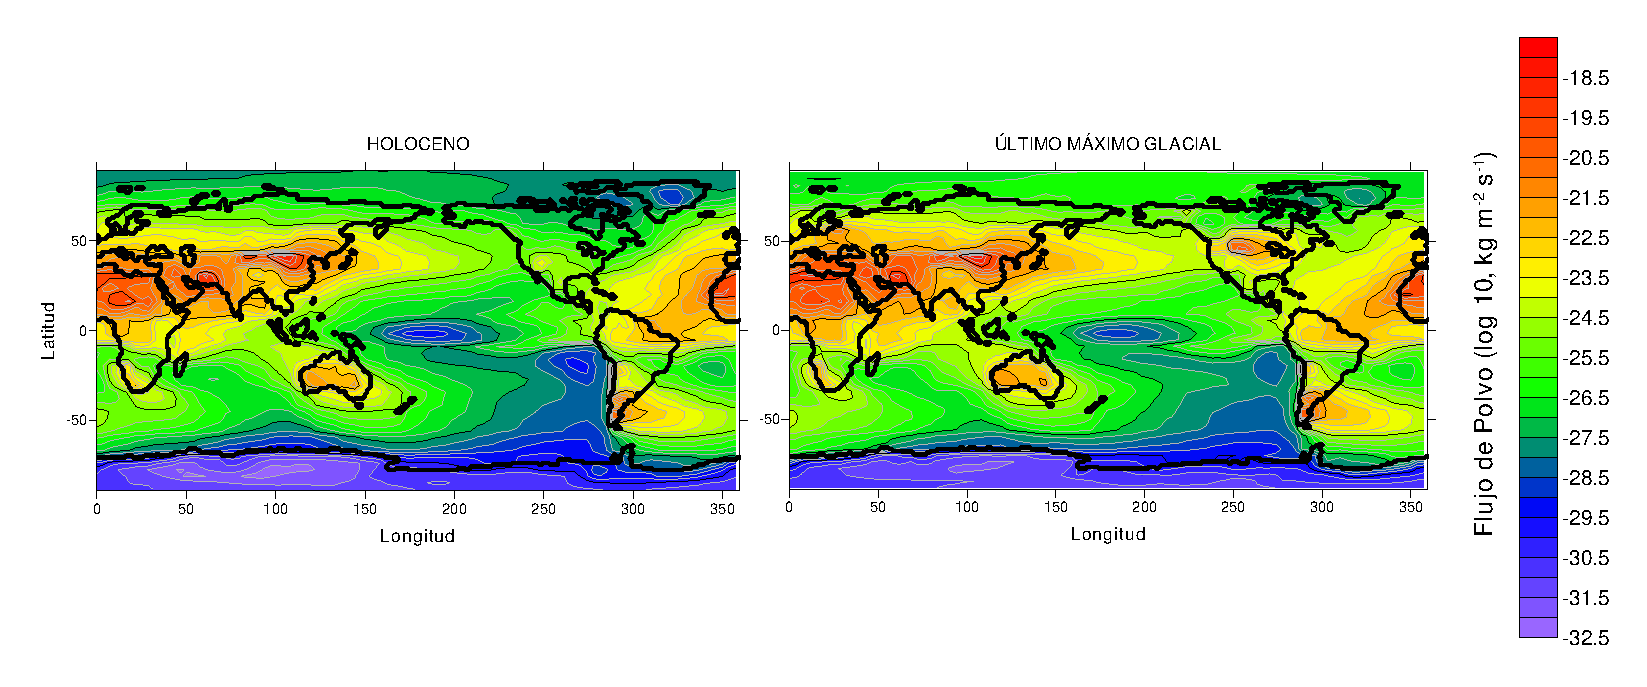
\includegraphics[width=1.1\textwidth]{Plot1_MRI.pdf}
  \caption[Flujos de polvo \cite{yukimoto2012new}]{Mapa global de flujos de polvo interpolados entre el periodo del Holoceno y el \'Ultimo M\'aximo Glacial. Datos obtenidos a partir \cite{yukimoto2012new}.}
  \label{fig:MRI}
\end{figure}

La depositación de polvo del modelo MRI-CGCM3, tanto en el Holoceno como en el UMG es de 2155.646  (Tg año$^{-1}$) para el Holoceno y 2965.467  (Tg año$^{-1}$) para el UMG. Donde las depositaciones de ambos periodos son similares, particularmente este efecto se aprecia en América del sur, donde durante el UMG no muestra flujo en la zona ecuatorial, mientras que en la zona patagónica existe un flujo que aporta en el Atlántico Sur, pero en general es similar al del Holoceno. 

 {\bf MIROC-ESM.} El modelo \textit{MIROC-ESM} perteneciente a PMIP3/CMIP5, fue desarrollado bajo el alero de los \textit{Earth system models} (ESMs) en la \textit{Japan Agency for Marine Earth Science and Technology} (JAMSTEC) en colaboración con el \textit{Center for Climate System Research} (CCSR), que estaban en búsqueda de un modelo que incluyera las retroalimentaciones del ciclo del carbono, es decir, que pudiera pronosticar las concentraciones de CO$_2$ atmosférico. Está basado en \textit{Model for Interdisciplinary Research on Climate} (MIROC3.2). MIROC-ESM es un modelo acoplado compuesto de un módulo de circulación atmosférica (MIROC-AGCM 2010), un módulo de circulación oceánica con una componente de hielo (COCO 3.4), un modelo de superficie de la tierra (MATSIRO), un módulo de aerosoles (SPRINTARS 5.00), y un componente de ecosistemas marinos (nutrientes, especies de plancton, NPZD) y terrestres (dinámica vegetacional, SEIB-DGVM), también se introduce una componente nueva relacionado con la química atmosférica (CHASER 4.1). Todos los módulos están conectadas mediante ``K-1'' un acoplador de flujo. 

Los datos de polvo presentados corresponden a la simulación de polvo MIROC-ESM en la que se utiliza el modelo \textit{Spectral Radiation-Transport Model for Aerosol Species} (SPRINTARS). El cual es un modelo físico tridimensional que predice la mezcla de los principales aerosoles troposféricos entre ellos: sulfato, polvo del suelo, carbonaceos (carbono orgánico (OC) y carbón (BC)), sal de mar, y precursores de gases de sulfato (dióxido de azufre (SO$_2$) y sulfuro de dimetilo (DMS)). Entre los procesos de transporte de estos gases está considerado la emisión, advección, difusión, química del azufre, deposición humeda, deposición seca y depositación gravitacional. El módulo es impulsado por un modelo de circulación atmosférica del CCSR que involucra procesos radiativos \citep{takemura2000global,sueyoshi2013set}.  

 \begin{figure}[H]
\centering
  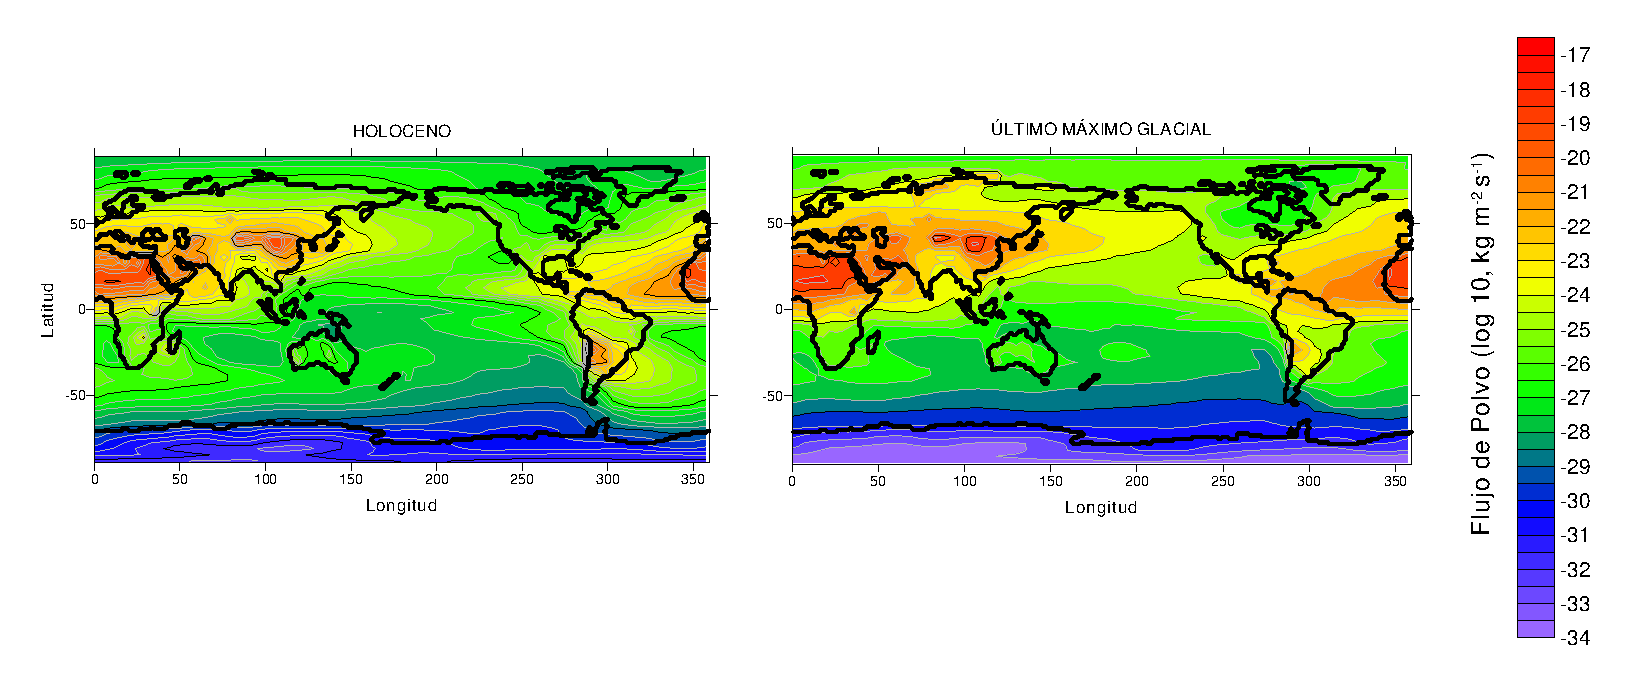
\includegraphics[width=1.1\textwidth]{Plot1_MIROC.pdf}
  \caption[Flujos de polvo \cite{sueyoshi2013set}]{Mapa global de flujos de polvo interpolados entre el periodo del Holoceno y el \'Ultimo M\'aximo Glacial. Datos obtenidos de \cite{sueyoshi2013set}.}
  \label{fig:MIROC}
\end{figure}

La depositación de polvo global simuladas por MIROC-ESM para el Holoceno y UMG, son de 2351.565 Tg año$^{-1}$ y 6674.501 Tg año$^{-1}$ respectivamente. 

Entre las bases de datos se puede apreciar un aumento de los flujos de polvo, habiendo una mayor producción durante el UMG que durante el Holoceno. No obstante, el modelo no presenta grandes fuentes de polvo en el Hemisferio Sur, lo que se refleja particularmente en la zona patagónica de Sur América, la cual es sabido es una importante fuente de polvo glaciogénico para los Océanos del Sur, de igual manera en la zona de Australia/Nueva Zelandia tampoco se aprecia una fuente de polvo. En las zona del Pacífico Ecuatorial si bien existe una lengua de polvo, es un aporte muy reducido.   

{\bf Takemura.} La distribuci\'on global de polvo presentado a continuaci\'on fue desarrollado a partir del modelo clim\'atico de aerosol SPRINTARS, junto con la inclusi\'on de la interacci\'on entre los cristales de hielo y las part\'iculas de aerosol. relacionados con la emisión de flujos de polvo aerosoles (velocidad del viento cercano a la superficie, de la cubierta vegetacional, y del índice folear, humedad del suelo y cantidad de nieve), así también las características relacionadas con el flujo de emisión de sal marina y la parametrización relacionada con la interacción entre los aerosoles y cristales de hielo. Para más detalle revisar el articulo de \cite{takemura2009simulation}.

\begin{figure}[H]
\centering
  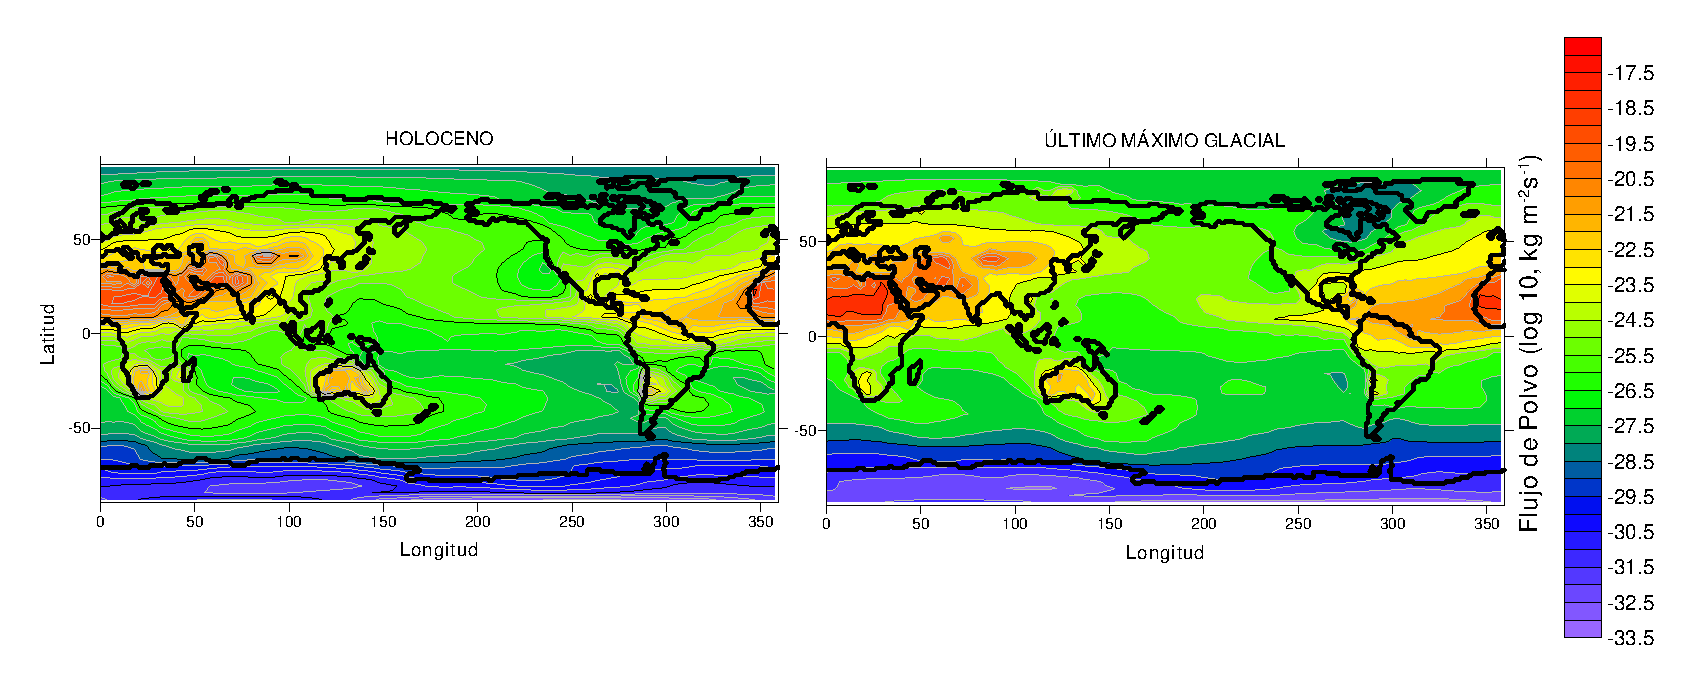
\includegraphics[width=1.1\textwidth]{Plot1_Takemura.pdf}
  \caption[Flujos de polvo \cite{takemura2009simulation}]{Mapa global de flujos de polvo interpolados entre el periodo del Holoceno y el \'Ultimo M\'aximo Glacial. Datos obtenidos de \cite{takemura2009simulation}.}
  \label{fig:Takemura}
\end{figure}

Los flujos de depositación globales de polvo a partir de esta simulación tienen valores de 2535.295 Tg año$^{-1}$ para el periodo del Holoceno y 5756.909 Tg año$^{-1}$ durante el UMG. Según \cite{takemura2009simulation} los flujos obtenidos se corresponden de buena manera con los datos de testigos de testigos de hielo y sedimentos marinos. Si bien durante el UMG la simulación mostró una expanción de las fuentes del Sahara hacia el sur y hacia el Norte sobre Europa del Este y Asia Central, hay una predominancia de altas tasas de deposición en latitudes altas del Hemisferio Norte mientras que en el Hemisferio Sur en zonas como la Antártica se aprecia una casi nula deposición (siendo que los datos muestran que hay una fuente primaria en la Patagonia), así mismo tanto Australia como África Austral muestran bajas tasas de depositación. 

{\bf Albani.} Para la construcción del campo de polvo ``\textit{Albani}'', se utilizó el modelo acoplado \textit{Community Earth System Model Version 1} (CESM1). El cual es un modelo de sistema tierra global incluido dentro de CMIP5, que está compuesto por cuatro módulos separados que representan la componente atmosférica, oceánica, de superficie terrestre y cubierta de hielo marina. Donde \citep{albani2014improved} hizo uso de la componente atmosférica, la \textit{Community Atmosphere Model version 4} (CAM4) y su versión posterior la \textit{Community Atmosphere Model version 5} (CAM5) (www.cesm.ucar.edu) ajustando para ello un conjunto de parametrizaciones físicas relacionadas con el polvo (erosibilidad del suelo, tamaño de distribución de polvo emitido, deposición húmeda y propiedades ópticas). Para la simulación de polvo del UMG se utilizó el subconjunto \textit{ Community Climate System Model} (CCSM4). Los resultados de las simulaciones son comparados con datos observacionales utilizando para ello el \textit{Aerosol optical depth} (AOD) en su versión 2, que da una estimación de la cantidad de haces de luz que se impide que lleguen a la superficie producto de la presencia de particulas de aerosoles en la columna de aire (como el polvo, la bruma, etc). Para la superficie se utilizó la concentración atmosférica y el flujo de deposición de polvo tomados de la \textit{University of Miami Ocean Aerosols Network}, también se utilizaron datos de estaciones, aunque estos últimos no fueron utilizados en la optimización de los modelos. 

\begin{figure}[H]
\centering
  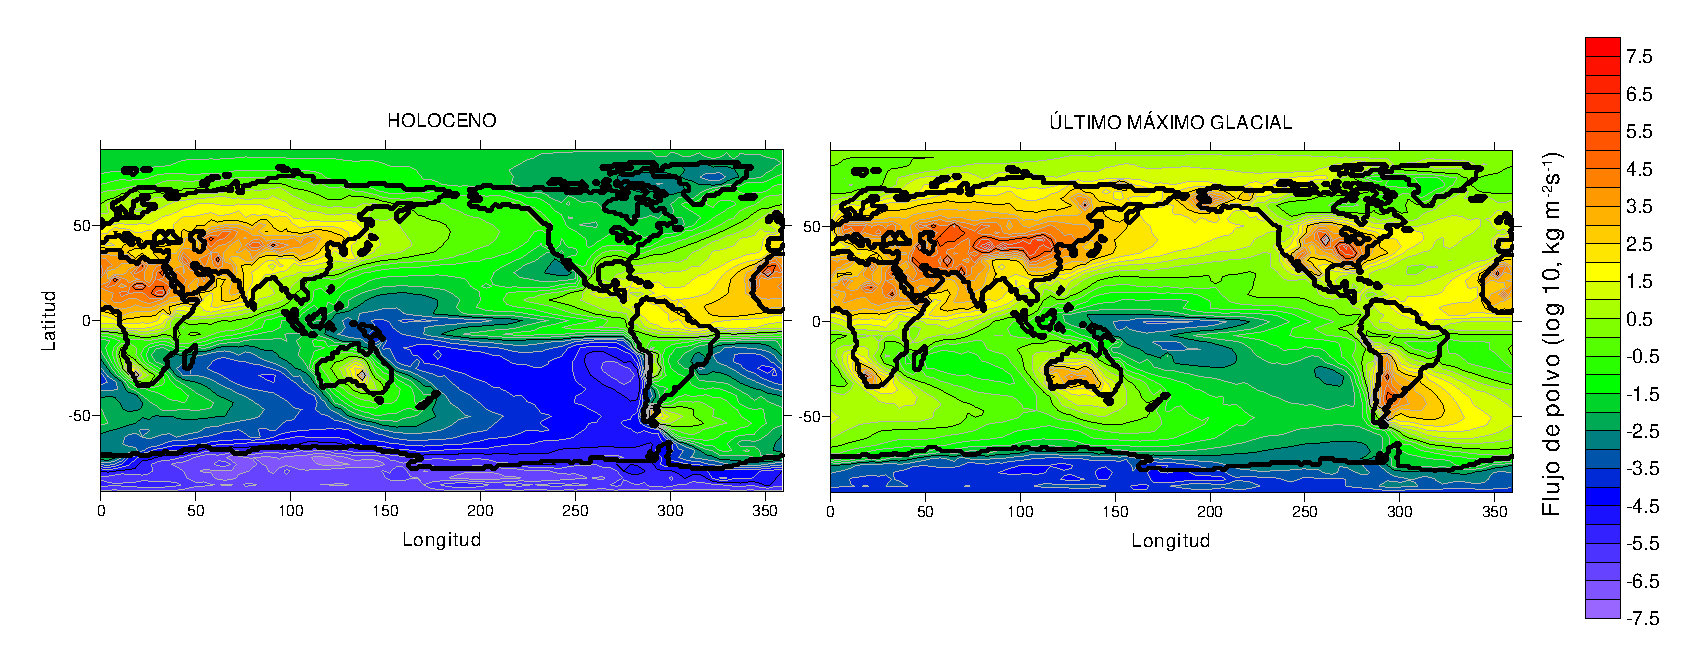
\includegraphics[width=1.1\textwidth]{Plot1_Albani.pdf}
  \caption[Flujos de polvo \cite{albani2014improved}]{Flujos de campos de polvo desarrollados mediante el modelo acoplado \textit{Community Earth System Model Version 1} (CESM1).  A la derecha el periodo del Último Máximo Glacial y a la izquierda el Holoceno. Datos obtenidos de \cite{albani2014improved}.}
  \label{fig:Albani}
\end{figure}

Los modelos tienden a mostrar altas emisiones con altas cargas, y periodos de vida más cortos durante el Holoceno en comparación a los datos de observaciones. Mientras que durante el UMG las magnitudes estimadas por el modelo son representativas de observaciones en paleo-datos en los 4 ordenes de magnitud abarcados por los datos. Donde alcanzan 2.2 veces lo calculado por unos de los modelos de 
\textit{Community Earth System Model Version 1} (CESM1), abarcando valores de $6289$ Tg/a. Además que el 20\% de las emisiones provienen de fuentes glaciogénicas, con una vida media de 2.2 días y una carga de polvo es 37.4 tg/año \citep{albani2014improved}. 


\subsection*{Análisis de datos}

Entre los campos de flujos de polvo las simulaciones realizadas por \cite{takemura2009simulation} (basada en el modelo \textit{MIROC-ESM}), reflejan una carencia de fuentes de polvo en el Hemisferio sur durante el UMG lo que se condice con el modelo \textit{MIROC-ESM}. No obstante, tanto \textit{MRI-CGCM3} como la reconstrucción \textit{Lambert} muestran un aumento en el aporte a esta zona en el UMG, mayormente en el Atlántico Sur, lo que los flujos de \textit{Albani} intensifican presumiblemente sobrestimando las concentraciones reales, pero mostrando la vital importancia de las fuentes glaciogenicas durante estos periodos. Por otro lado, todas las simulaciones y reconstrucción exponen una considerable intensificación de las fuentes de polvo en el Hemisferio Norte en el UMG, siendo \textit{Lambert} uno de los que más diferencias muestran en esta zona (ver imagen \ref{fig:Amp}). Además respecto de la zona del Pacífico Ecuatorial, tanto \textit{MIROC-ESM} y \textit{Takemura} revelan altas depositaciones durante el UMG, sin embargo, es en la zona este de la región donde se aprecia una lengua de depositación de polvo que es compartida por todos los modelos. 

\section{Pre-procesamiento}

\begin{figure}[H]
\centering
  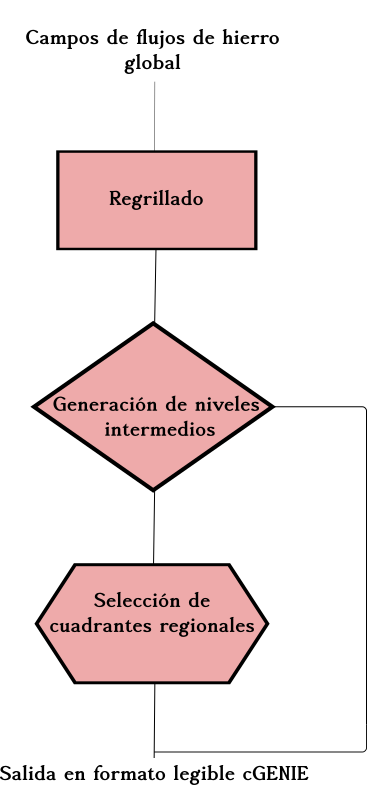
\includegraphics[width=0.29\textwidth]{diagrama_met1.png}
  \caption[Pre-procesamiento de datos]{Estructura del pre-procesamiento de los flujos de campo de polvo.}
  \label{fig:diagrama_met1}
\end{figure}

En esta etapa se realizan tres procesos diferentes que serán posteriormente utilizados como input en el modelo cGENIE: 1) la redimención de campos de polvo globales de los periodos del Holoceno y LGM, 2) la generación de niveles intermedios equidistantes entre los periodos anteriores y 3) la generación de campos regionales desde el campo intermedio posterior al Holoceno hasta el UMG. 

\begin{description}
  \item[1) Regrillado de campos de polvo globales Holoceno y UMG:]

Los 5 campos de polvo expuestos en la sección 4.1 para el Holoceno y para el UMG, tienen una grilla que es de 128x64 celdas en cuatro casos (Lambert, Takemura, MIROC-ESM, MRI-CGCM3) y una de 192x268 celdas (Albani). Para el modelo cGENIE es necesario traspasar todos los campos a una grilla cuadrada de 36x36, que serán los nuevos campos de flujos de polvo globales tanto para el Holoceno (5 campos) y para el UMG (5 campos). 

  \item[2) Campos de polvo intermedios globales Holoceno y UMG:]

Con el propósito de observar los cambios en la concentración de CO$_2$ atmosférico que se dan entre el periodo del Holoceno hasta el UMG, y sobre la base de los diferentes inputs de campos de polvo previamente regrillados (\textit{item 1}), se realiza una interpolación x-espaciada, creando con ello 8 diferentes escenarios intermedios de polvo. Éstos en conjunto con el \textit{item 1} generan 10 niveles que van desde el Holoceno hasta el UMG incluyendo ambos periodos.

   \item[3) Campos de polvo intermedios regionales:]

Para ver el efecto que cada zona HNLC (ver figura \ref{fig:Grilla4}) aporta en la captura de pCO$_2$ producto de la fertilización con hierro, se procedió a generar nuevos campos de polvo a partir de los 10 producidos de la combinación del \textit{item 1 e item 2}. 

Para ello, en primera instancia la concentración de polvo correspondiente al Holoceno (nivel 1) se inserta en cada punto de grilla que no tenga asociada una zona HNLC de interés (dejando su concentración original), este proceso se reproduce en todos los niveles de polvo de la misma forma (hasta el niveles 10). Ésto produce 10 campos de polvo donde la única variación de polvo a lo largo del tiempo (que abarca el Holoceno y UMG) se da en la zona HNLC seleccionada (manteniendo sus datos originales en todos los niveles). Este proceso se replica para cada zona HNLC, generando finalmente 10 campos de polvo por región, es decir, 40 campos de polvo por casa caso (Albani, Lambert, MIROC-ESM, MRI-CGCM3, Takemura). 
\end{description}

\subsection{Pre-procesamiento modelo cGENIE}

Una vez generados los flujos de campos de polvo globales desde el Holoceno hasta el UMG y los flujos de polvo intermedios, se procede a subir los archivos en la configuración de cGENIE ejecutado en un cluster de la Universidad de BRISTOL.

\begin{figure}[H]
\centering
  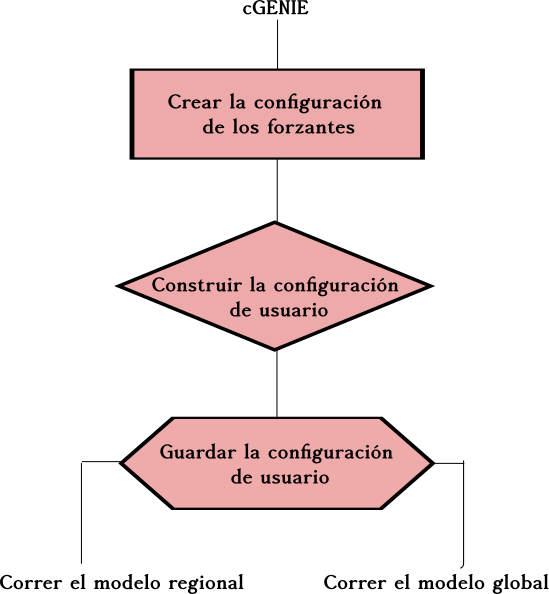
\includegraphics[width=0.5\textwidth]{diagrama_met2.png}
  \caption[Pre-procesamiento modelo cGENIE]{Estructura del pre-procesamiento de los flujos de campo en cGENIE.}
  \label{fig:diagrama_met2}
\end{figure}

 Para configurar un experimento en el modelo cGENIE, es necesario ingresar en el directorio localizado en cgenie.muffin/genie-forcings, dado que aqu\'i es donde son almacenado los forzantes y contiene todos los archivos que definen las propiedades geoqu\'imicas que modificaran la informaci\'on acerca de como un forzante cambiar\'a en el tiempo. En este caso el trazador corresponde a los campos de flujos de polvo generados en el \textit{item 1/item f2 e item3} de la secci\'on 4.2. Se especifican los cambios en las concentraciones del forzante en el tiempo ``Condiciones de contorno del modelo''. 

 Así, en este caso se crearon manualmente dos carpetas en genie-forcings, una con el nombre ``worjh2.FeMODELO\_All.level*'' y otra llamada ``worjh2.FeMODELO\_Regi\'on.level*'', para simulaciones globales y regionales respectivamente. Esto se replic\'o para todos los niveles de polvo en cada caso. 

Dentro de cada una de estas carpetas se incorporaron 5 archivos: 

\begin{itemize}
  \item[1) ] \textbf{biogem\_force\_flux\_sed\_det\_SUR.dat} ``biogem\_force\_*\_I.dat''. Especifica la ubicación en el océano del forzante geoquímico que será aplicado (componente espacial). En este caso la grilla de flujo de polvo es de dos dimensiones (grupos de datos que contienen filas (j) y columnas (i)), en unidades de mol a$^-1$. 
  \item[2) ] ``configure\_forcings\_atm.dat''. Definición de forzantes atmosféricos interactuando en el modelo. Para esta simulación no se definen. 
  \item[3) ] ``configure\_forcings\_ocn.dat''.Definición de forzantes oceánicos interactuando en el modelo. En esta simulación no se definen. 
  \item[4) ] ``\textbf{configure\_forcings\_sed.dat}''. Definición de forzantes sedimentarios interactuando en el modelo. Para esta simulación se definen forzantes provenientes de sedimentos terrestres (polvo). 
  \item[5) ] biogem\_force\_flux\_sed\_det\_sig.dat ``biogem\_force\_*\_II.dat''. Define la componente temporal del forzante (variación en el tiempo). 
Se construye a partir de la magnitud del forzante que es aplicado en la posición $(i,j)$ en un tiempo $_{(t)}$, m\'as un modificador S$_{(t)}$ que es dependiente del tiempo, por la diferencia entre los dos campos \textit{item 5 - item 1}, es decir: 
 \begin{equation} \label{eq:met1}
F_{(i,j),(t)}= biogem\_force\_*\_I_{(i,j)}\ +\ S_{(t)}\ \times\ (biogem\_force\_*\_II_{(i,j)}\ -\ biogem\_force\_*\_I_{(i,j)})
\end{equation}
El valor del trazador de escala ($S_{(t)}$) es interpolado desde los contenidos de la se\~nal forzante del archivo 
biogem\_force\_flux\_sed\_det\_SUR.dat.
\end{itemize}

Luego de crear las carpetas y archivos para todos los niveles de polvo y para cada tipo (regional o global), es que se crearon los archivos y carpetas de configuraci\'on (ver figura Anexo \ref{tabla:U-conf}). Este proceso se realiza en el directorio \textit{genie-Userconfig} dentro del directorio \textit{cgenie.muffin}. \newpage

\section{Experimento, modelo cGENIE}

 \begin{figure}[H]
\centering
  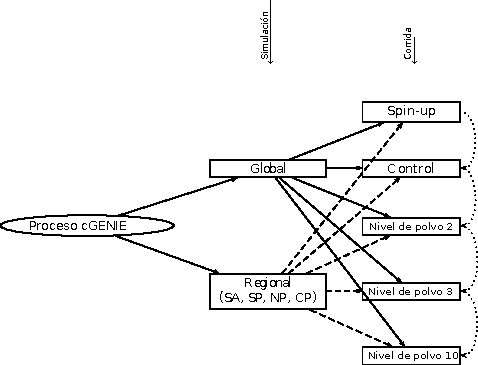
\includegraphics[width=0.7\textwidth]{runcGENIEpdf.pdf}
  \caption[Estructura de la Simulación en cGENIE]{Estructura de la Simulación en cGENIE. Se aprecia el Spin-up (configuración básica) para posteriormente representar la evaluación progresiva de los flujos de polvo.}
  \label{fig:run}
\end{figure}

La simulación fue desarrollada en tres etapas: 1) se realiz\'o una configuración básica necesaria para dar una consistente iniciación al modelo cGENIE (spin-up), 2) se ejecut\'o una simulación de control para verificar que el modelo ratifique los valores observados y 3) se evaluaron los niveles de campos de polvo desde el Holoceno hasta el UMG en todos los casos dados (globales y regionales). 

\subsection*{Configuración general}

Todos las simulaciones que se expondrán a continuación (spin-up, control, experimentos), fueron corridos por un intervalo de tiempo de 10000 años (para la estabilización, figura \ref{fig:Control}). En este caso, dado que buscamos evaluar el efecto del hierro en la bomba biológica y cómo esto afecta la concentración de CO$_2$, la componente de biogeoquímica oceánica correspondiente al módulo BIOGEM toma una importante relevancia. Mientras que la configuración básica seleccionada es \textit{cgenie.eb\_go\_gs\_ac\_bg.worjh2.BASEFe}, la cual representa los módulos presentes en la tabla \ref{tabla:Met1}, la configuración continental, la resolución y trazadores escogidos incluyendo el ciclo del hierro marino. 

\begin{description}
\item[1) Spin-up:] Con el propósito de establecer las parametrizaciones del modelo cGENIE en las condiciones climatológicas del periodo preindustrial es que se desarrolla un spin-up. Para lo cual, se utilizó el flujo de polvo del Holoceno de cada modelo/reconstrucción de polvo. En esta etapa se fija el CO$_2$ en 278 ppm (concentración periodo preindustrial), con un ``biogem\_force\_*\_II.dat'' fijado en cero lo que significa que no tomará los valores del forzante de polvo que le estamos ingresando (ver figura \ref{fig:SPIN-UP}). 

De aquí en adelante todos los experimentos fueron corridos dependiendo del final del estado del spin-up. 

\item[2) Control:] Se desarroll\'o una simulación de control aplicando los mismo campos de polvo usados por el Spin-up (Holoceno), pero sin fijar la concentración atmosférica de CO$_2$. La figura \ref{fig:Control} de las simulaciones de control, muestra una estabilización alrededor de los 2000 años para todos los modelos y reconstrucciones.

\item[3) Experimentos:] Finalmente procedemos a correr el modelo desarrollando tantos las evaluaciones del efecto del hierro en la captura de CO$_2$ a nivel global como regional (zonas HNLC).
En la l\'inea de comando del cluster BRISTOL, dentro del directorio genie-main ingresamos el comando: ( \$ qsub -j y -o cgenie\_log -V -S /bin/bash runmuffin.sh ) junto con una lista de parámetros que permiten correr el modelo.\\
\$... ./runmuffin \#1 \#2 \#3 \#4 (\#5)

Estos par\'ametros son:\\
\#1 el nombre de la configuraci\'on b\'asica requerida para el modelo, en este caso ser\'a\\
\textit{cgenie.eb\_go\_gs\_ac\_bg.worjh2.BASEFe}.\\
\#2 nombre del subdirectorio que contiene los archivos ``user-config'', en nuestro caso ``DUST''. \\
\#3 nombre del archivo de configuraci\'on (user-config).\\
\#4 longitud de la corrida en a\~nos, en nuestro caso 10000 a\~nos. Para el caso del \textit{spin-up} s\'olo se ocupan los par\'ametros definidos hasta aqu\'i.  \\ 
\#5 corrida de arranque (periodo preindustrial), en nuestro caso ``worjh2.PO4Fe.SPIN''. Necesario para la simulaci\'on de control y experimento con polvo. 

Al finalizar la corrida los archivos de salida (resultados) son almacenados dentro del directorio \textit{cgenie\_output}. 
\end{description}

\begin{figure}[H]
\centering
 \includegraphics[width=1.2\textwidth]{../../Figuras/Series/Series_Holoceno.png}
 \caption[Series de pCO$_2$ de simulación de control]{Serie de tiempo de pCO$_2$ obtenidos a partir de las simulaciones de control realizadas mediante el modelo cGENIE, para el periodo del Holoceno de todos los campos de polvo.}
  \label{fig:Control}
\end{figure}

\section{Post-procesamiento}

Los archivos de $pCO_2$ obtenidos del modelo cGENIE, son procesados en el software \textit{Matlab} en el cual se procede de la siguiente manera: 

\begin{itemize}
    \item[a) ] Se seleccionaron los últimos 10 datos del archivo biogem\_series\_atm\_pCO2.res ubicado en cgenie\_output/user\_config/biogem, correspondientes a niveles de pCO$_2$ de la parte estable de la simulación. 
    \item[b) ] Sacamos la diferencia de pCO$_2$ entre cada nivel desde el periodo preindustrial (nivel 1) hasta el \'Ultimo M\'aximo Glacial (nivel 10).
    \item[c) ] En el caso del flujo global, se hiz\'o una mediana del pCO$_2$ obtenido con cGENIE, para los 10 periodos (niveles).
    \item[d) ] Posteriormente se graficaron las diferencias de $pCO_2$ respecto del hierro en cada nivel y se ajust\'o una curva a los datos.
    \item[e) ] Por otro lado, se calculó en porcentaje la reducción de cada nivel para cada zona
de interés respecto del UMG. De esta manera, se obtuvo un porcentaje relativo del aporte de cada zona HNLC a la reducción total de CO$_2$ (ver Anexos) para cada modelo y recontrucción ingresada en cGENIE.
\end{itemize}



